\section{Establishing the Eigenfunction Property}

% Prove that the 2 eigenfunctions are, indeed, Fourier eigenfunctions!

In this section, we show that the $\pm$-Eigenfunctions are, indeed, $\pm$-Eigenfunctions of the Fourier transform.

In the previous section, we did not work with $a$ and $b$ directly as it was sufficient to work with $a\rad$ and $b\rad$ instead. In this section, however, we will need to use the following formula for the $n$-dimensional Fourier transform of the $n$-dimensional Gaussian.

\begin{boxtheorem}[Fourier Transform of a Gaussian]\label{Ch4:Thm:GaussianFourier}
    Fix $n \in \N$ and $b \in \C$, with $\Re(b) > 0$. If $F : \R^n \to \C$ is given by
    \begin{align*}
        F(x) = e^{-b \norm{x}^2}
    \end{align*}
    then the Fourier transform of $F$ is given by
    \begin{align*}
        \hat{F}\of{\omega} = \parenth{\frac{\pi}{b}}^{{n} / {2}} e^{{- \pi^2 \norm{\omega}^2} / {b}}
    \end{align*}
\end{boxtheorem}
A \href{https://github.com/leanprover-community/mathlib4/blob/5a2eaa85c555c4263e15928cef249cbaad2eb2d2/Mathlib/Analysis/SpecialFunctions/Gaussian/FourierTransform.lean#L360-L363}{formal proof} exists in \mathlib.

We will also need the following version of the \CGT, which allows us to deform contours of integration in the complex plane.

\begin{boxtheorem}[Cauchy-Goursat: Squares and Circles]\label{Ch4:Thm:CGTRectCircle}
    Fix $w \in \C$ and $r > 0$. Let $\gamma$ be the quarter-circle parametrised by $\gamma(t) = w + r\pcos{t} + \abs{r} i \psin{t}$ for $0 \leq t \leq \pi/2$. For any $f : \C \to \C$ that is holomorphic in the region enclosed by $\gamma$ and the line segments from $w + r$ to $w + r + ir$ and $w + r + ir$ to $w + ir$, we have
    \begin{align*}
        \int_{\gamma} f(z) \, \diff{z}
        = \int_{w + r}^{w + r + ir} f(z) \, \diff{z} + \int_{w + r + ir}^{w + ir} f(z) \, \diff{z}
    \end{align*}
\end{boxtheorem}

While this is an immediate consequence of the more general (and well-known) \CGT\ from complex analysis, there are numerous challenges involved in formalising this and other versions of the theorem. We will discuss it in \Cref{Ch5:Sec:Cauchy-Goursat}. We also note that the above result implies an analogous result for 

\begin{figure}[ht]
    \centering
    \begin{subfigure}{0.48\linewidth}
        \centering
        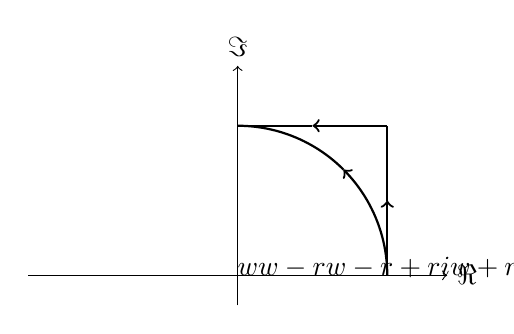
\begin{tikzpicture}[scale=1.9]
            % Axes
            \draw[->] (-1.4,0) -- (1.4,0) node[right] {$\Re$};
            \draw[->] (0,-0.2) -- (0,1.4) node[above] {$\Im$};
        
            % Quarter-circle contour
            \draw[thick, domain=0:45, ->] plot ({cos(\x)}, {sin(\x)});
            \draw[thick, domain=45:90, -] plot ({cos(\x)}, {sin(\x)});

            % Rectangular contour
            \draw[thick, ->] (1,0) -- (1,0.5);
            \draw[thick, -] (1,0.5) -- (1,1);
            \draw[thick, ->] (1,1) -- (0.5,1);
            \draw[thick, -] (0.5,1) -- (0,1);

            % Points of interest
            \labelledpoint{0}{0}{-0.3}{-0.8}{$w$}
            \labelledpoint{1}{0}{0}{-0.8}{$w - r$}
            \labelledpoint{1}{1}{0.3}{-0.2}{$w - r + ri$}
            \labelledpoint{0}{1}{-0.7}{-0.5}{$w + ri$}
        \end{tikzpicture}
        \caption{Contours for which \Cref{Ch4:Thm:CGTRectCircle} holds.}
    \end{subfigure} 
    \hfill
    \begin{subfigure}{0.48\linewidth}
        \centering
        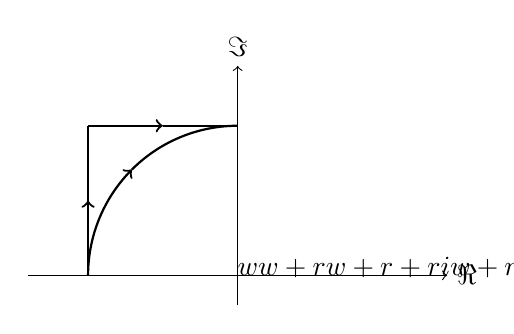
\begin{tikzpicture}[scale=1.9]
            % Axes
            \draw[->] (-1.4,0) -- (1.4,0) node[right] {$\Re$};
            \draw[->] (0,-0.2) -- (0,1.4) node[above] {$\Im$};
        
            % Quarter-circle contour
            \draw[thick, domain=180:135, ->] plot ({cos(\x)}, {sin(\x)});
            \draw[thick, domain=135:90, -] plot ({cos(\x)}, {sin(\x)});

            % Rectangular contour
            \draw[thick, ->] (-1,0) -- (-1,0.5);
            \draw[thick, -] (-1,0.5) -- (-1,1);
            \draw[thick, ->] (-1,1) -- (-0.5,1);
            \draw[thick, -] (-0.5,1) -- (0,1);

            % Points of interest
            \labelledpoint{0}{0}{0.3}{-0.8}{$w$}
            \labelledpoint{-1}{0}{0}{-0.8}{$w + r$}
            \labelledpoint{-1}{1}{-0.3}{-0.2}{$w + r + ri$}
            \labelledpoint{0}{1}{0.7}{-0.5}{$w + ri$}
        \end{tikzpicture}
        \caption{Contours for which an analogous result holds.}
        \label{Ch4:Subfig:CGTRectCircle_Alt}
    \end{subfigure} 
    \caption{The contour deformations permitted by \Cref{Ch4:Thm:CGTRectCircle}.}
\end{figure}

We now prove that $a$ is indeed a $+1$-eigenfunction of the Fourier transform.

\subsection{The $+1$-Eigenfunction}

The Fourier transform acts very interestingly on $a$. Recall from \Cref{Ch3:Thm:FourierSchwartz_CLE} that the Fourier transform is a linear isomorphism of Schwartz spaces. Since $I_1, \ldots, I_6$ are Schwartz, so are their compositions with the norm-squared function. Hence, for all $x \in \R^8$,
\begin{align*}
    \F\of{a(x)}
    % = \F\of{I_1\of{\norm{x}^2}} + \F\of{I_2\of{\norm{x}^2}} + \F\of{I_3\of{\norm{x}^2}} + \F\of{I_4\of{\norm{x}^2}} + \F\of{I_5\of{\norm{x}^2}} + \F\of{I_6\of{\norm{x}^2}}
    = \F\of{\sum_{j=1}^{6} I_j\of{\norm{x}^2}}
    = \sum_{j=1}^{6} \F\of{I_j\of{\norm{x}^2}}
\end{align*}

The strategy to show that $\F\of{a} = a$ will be to show that $\F$ acts on the $I_j\of{\norm{x}^2}$ in the following manner:\footnote{Note that we are abusing notation by denoting the function $x \mapsto I_j\of{\norm{x}^2} \in \Sch\of{\R^8, \C}$ by $I_j\of{\norm{x}^2}$.}
\begin{align}
    \F\of{I_1\of{\norm{x}^2} + I_2\of{\norm{x}^2}} &= I_3\of{\norm{x}^2} + I_4\of{\norm{x}^2} \label{Ch4:Eq:a_is_eig_perm_12_34} \\
    \F\of{I_3\of{\norm{x}^2} + I_4\of{\norm{x}^2}} &= I_1\of{\norm{x}^2} + I_2\of{\norm{x}^2} \label{Ch4:Eq:a_is_eig_perm_34_12} \\
    \F\of{I_5\of{\norm{x}^2}} &= I_6\of{\norm{x}^2} \label{Ch4:Eq:a_is_eig_perm_5_6} \\
    \F\of{I_6\of{\norm{x}^2}} &= I_5\of{\norm{x}^2} \label{Ch4:Eq:a_is_eig_perm_6_5}
\end{align}
Since, in addition to being Schwartz, all the $I_j\of{\norm{x}^2}$ (and their sums) are radial, \Cref{Ch3:Prop:RadialSchwartzFourier} tells us that \eqref{Ch4:Eq:a_is_eig_perm_34_12} and \eqref{Ch4:Eq:a_is_eig_perm_6_5} follow from \eqref{Ch4:Eq:a_is_eig_perm_12_34} and \eqref{Ch4:Eq:a_is_eig_perm_5_6} respectively. We now prove \eqref{Ch4:Eq:a_is_eig_perm_12_34} and \eqref{Ch4:Eq:a_is_eig_perm_5_6}.

\begin{boxlemma}
    The Fourier transform % $\F : \Sch\of{\R^8, \C} \to \Sch{\R^8, \C}$
    maps $I_1\of{\norm{x}^2} + I_2\of{\norm{x}^2}$ to $I_3\of{\norm{x}^2} + I_4\of{\norm{x}^2}$.
\end{boxlemma}
\begin{proof}
    It has been formally verified that \href{https://github.com/leanprover-community/mathlib4/blob/5a2eaa85c555c4263e15928cef249cbaad2eb2d2/Mathlib/Analysis/Fourier/FourierTransform.lean#L360-L362}{the Fourier integral of a function converges absolutely iff the function is integrable} and that \href{https://github.com/leanprover-community/mathlib4/blob/5a2eaa85c555c4263e15928cef249cbaad2eb2d2/Mathlib/Analysis/Distribution/SchwartzSpace.lean#L1095-L1097}{Schwartz functions are integrable}. Hence, \href{https://github.com/leanprover-community/mathlib4/blob/5a2eaa85c555c4263e15928cef249cbaad2eb2d2/Mathlib/Analysis/Distribution/FourierSchwartz.lean#L36}{the Fourier integral of a Schwartz function converges absolutely}. Since 
    % The problem I have is that what's in mathlib tells me that Fourier integral of I_1 converges absolutely, but not that the integral with respect to the product measure on R^8 and [0,1] of the integrand of I_1 converges absolutely.
\end{proof}

\subsection{The $-1$-Eigenfunction}